\chapter{Leis de Maxwell e Ondas Eletromagnéticas} \label{chap:maxwell}


As Leis de Maxwell constituem o arcabouço fundamental da eletrodinâmica clássica, unificando os fenômenos elétricos e magnéticos em um sistema coerente de equações diferenciais. Neste capítulo, exploramos essas equações em sua forma integral e diferencial, discutindo suas implicações físicas e derivando a equação de onda eletromagnética no vácuo.

\section{Equações de Maxwell}

As equações de Maxwell no vácuo podem ser escritas na forma diferencial como:

\begin{align}
  \nabla \cdot \vec{E} &= \frac{\rho}{\varepsilon_0} && \text{(Lei de Gauss para o campo elétrico)} \label{eq:maxwell1} \\
  \nabla \cdot \vec{B} &= 0 && \text{(Lei de Gauss para o campo magnético)} \label{eq:maxwell2} \\
  \nabla \times \vec{E} &= -\frac{\partial \vec{B}}{\partial t} && \text{(Lei de Faraday)} \label{eq:maxwell3} \\
  \nabla \times \vec{B} &= \mu_0 \varepsilon_0 \frac{\partial \vec{E}}{\partial t} && \text{(Lei de Ampère-Maxwell)} \label{eq:maxwell4}
\end{align}

Onde:
\begin{itemize}
    \item $\vec{E}$ e $\vec{B}$ são os campos elétrico e magnético, respectivamente;
    \item $\rho$ é a densidade de carga;
    \item $\varepsilon_0$ é a permissividade elétrica do vácuo; e
    \item $\mu_0$ é a permeabilidade magnética do vácuo.
\end{itemize}

A forma integral das mesmas equações é dada por:

\begin{align}
  \oint_{\mathcal{S}} \vec{E} \cdot d\vec{A} &= \frac{Q_{\text{int}}}{\varepsilon_0} \label{eq:maxwell-int1} \\
  \oint_{\mathcal{S}} \vec{B} \cdot d\vec{A} &= 0 \label{eq:maxwell-int2} \\
  \oint_{\partial \mathcal{S}} \vec{E} \cdot d\vec{l} &= -\frac{d}{dt} \int_{\mathcal{S}} \vec{B} \cdot d\vec{A} \label{eq:maxwell-int3} \\
  \oint_{\partial \mathcal{S}} \vec{B} \cdot d\vec{l} &= \mu_0 \varepsilon_0 \frac{d}{dt} \int_{\mathcal{S}} \vec{E} \cdot d\vec{A} \label{eq:maxwell-int4}
\end{align}

\section{Velocidade da Luz}

A partir da equação de onda, a velocidade de propagação no vácuo é:
\[
  c = \frac{1}{\sqrt{\mu_0 \varepsilon_0}}
\]

Com os valores experimentais de \eqref{eq:dados-experimentais}, obtemos \( c = \qty{299792458}{\meter\per\second} \).

\begin{equation} \label{eq:dados-experimentais}
    \begin{split}
        \varepsilon_0 &= \qty{8.854187817e-12}{\farad\per\meter} \\
        \mu_0 &= 4\pi \times \qty{e-7}{\henry\per\meter}
    \end{split}
\end{equation}


\section{Representação Gráfica da Onda Eletromagnética}

\begin{figure}[h]
  \centering
  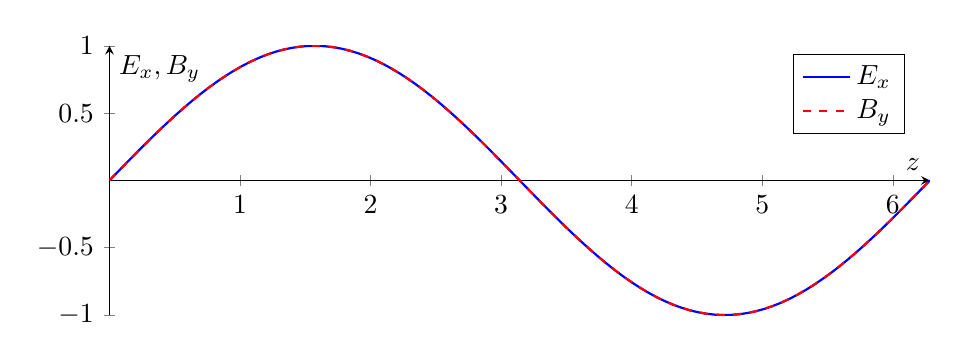
\begin{tikzpicture}
    \begin{axis}[
      axis lines=middle,
      xlabel={$z$},
      ylabel={$E_x, B_y$},
      samples=100,
      width=12cm,
      height=5cm,
      legend pos=north east,
      domain=0:2*pi
    ]
      \addplot[blue, thick] {sin(deg(x))};
      \addplot[red, thick, dashed] {sin(deg(x))};
      \legend{$E_x$, $B_y$}
    \end{axis}
  \end{tikzpicture}
  \caption{Ondas elétricas ($E_x$) e magnéticas ($B_y$) propagando-se ao longo do eixo $z$ com mesma fase.}
  \label{fig:onda_em}
\end{figure}
